\chapter{LÍNEAS FUTURAS\label{sec:lineasfuturas}}

\clearpage

Finalmente, con el entendimiento del estado actual de las tecnologías usadas en las app para emergencias, otro punto también a destacar es el planteamiento del posible futuro de estas apps si se integrase un servicio de mensajería instantánea.

\section{Servicios avanzados de PEMEA}

Los primeros resultados del proyecto, junto con las pruebas realizadas, confirman el poder de PEMEA para proporcionar:

\begin{itemize}
  \item Ciudadanos con acceso a servicios de emergencia en cualquier lugar de Europa utilizando sus apps locales en roaming.
  \item Los PSAPs con la información correcta (ubicación precisa, idioma de la persona que llama, contactos de ICE, etcétera), independientemente de la app que la persona esté utilizando.
\end{itemize}

En una segunda etapa, los servicios de emergencia se beneficiarán de los servicios avanzados de PEMEA, como geolocalización, compartición de imágenes y vídeos, o comunicación en tiempo real, para mejorar el acceso a los ciudadanos que presentan algún tipo de discapacidad y personas dependientes.

Deveryware ya ha invertido en este campo 3 años de investigación y experimentación.

\section{Soluciones WebRTC}

En resumen, la tecnología SIP es una gran manera de mejorar la comunicación, ya que ofrece una solución más barata y de alta calidad. Pero, de manera similar a como SIP ha reemplazado a la telefonía tradicional, WebRTC va a reemplazar a SIP debido a sus limitaciones. WebRTC proporciona aún mejor calidad con total flexibilidad. Además, los precios, comparados con el número de ventajas que proporciona, pueden parecer ridículos y no requieren una inversión inicial \cite{webrtc2}.

Por eso mismo, cada vez son más las empresas que optan por ofrecer servicios WebRTC y cada vez son más los clientes que apuestan por ellas, poco a poco están ganando el público que las centralitas SIP anteriormente robaron a las centralitas tradicionales \cite{webrtc1}.

\subsection{HYDRA}

Hydra, al tratarse de ACD basado en tecnología WebRTC, es accesible a través de cualquier dispositivo conectado a internet, ya sea un PC, una tablet e incluso una Smart TV, posibilitando conectarse desde la oficina, desde casa y en cualquier parte del mundo \cite{webrtc4}.

\begin{figure}[htp!]
  \centering
  
\includegraphics[scale=0.1,clip=true]{hydra_logo}
  \caption{Logo de HYDRA}
  \label{fig:hydra_logo}
\end{figure}

Tiene muchas funcionalidades sobre la tecnología WebRTC, entre las cuales se destaca las que sería interesante añadir a los PSAPs:

\begin{itemize}
  \item \textbf{Reconocimiento del lenguaje natural}. El uso de sistemas de reconocimiento del lenguaje natural te permite, como responsable del servicio, tener total control del contenido de las conversaciones recibidas o realizadas sobre cualquiera de los números de la empresa, por cualquiera de los empleados o agentes, independientemente de dónde se ubiquen o qué dispositivo utilizan. Además de poder recibir una transcripción de cada llamada, puede también recibir una traducción de la misma. Puedes elegir entre diferentes patrones de detección y analizar cualquier conversación sin importar el lenguaje utilizado en la misma \cite{webrtc4}.
  \item \textbf{Grabación de llamadas}. Grabación de llamadas entrantes y salientes. Grabación total o parcial de las llamadas.
  \item \textbf{Control avanzado de la voz}. Sistema biométrico de identificación de voz. Análisis del vocabulario y del estado emocional durante la conversación.
  \item \textbf{Monitorización de llamadas}. Auditar en tiempo real a sus agentes o su centro de llamadas. Intervenir llamadas o realizar escuchas durante las mismas para indicar a sus agentes cómo deben atender a sus clientes.
\end{itemize}

\section{Chatbots}

Hoy en día las apps de mensajería están convirtiéndose en uno de los servicios más utilizados por los usuarios de dispositivos móviles. Por esta razón, varios sectores están incorporando estos canales a sus modelos de negocio, un servicio que no estará controlado por personas, sino por robots \cite{chatbot2}.

En este sentido, tanto editores como apps de mensajería están centrando todos sus esfuerzos en el desarrollo de softwares de inteligencia artificial para crear chatbots, es decir, bots capaces de entablar conversaciones con los usuarios.

Un bot es un software de inteligencia artificial diseñado para realizar una serie de tareas por su cuenta y sin la ayuda del ser humano \cite{chatbot1}.

\begin{figure}[htp!]
  \centering
  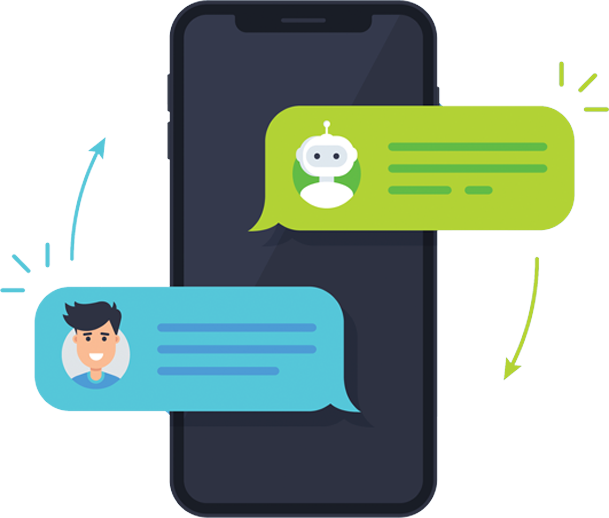
\includegraphics[scale=0.2,clip=true]{chatbot}
  \caption{Chatbot}
  \label{fig:chatbot}
\end{figure}

Los chatbots son un tema candente en estos días. Los conjuntos de herramientas disponibles han permitido a muchas empresas integrar con éxito la tecnología de chatbot en sus sistemas empresariales, ahorrando tiempo y dinero.

Una de las grandes ventajas de los chatbots es que, a diferencia de las aplicaciones, no se descargan, no es necesario actualizarlos y no ocupan espacio en la memoria del teléfono \cite{chatbot3}.

Otros lugares en los que han estado en funcionamiento en los últimos años ha sido en chats como Facebook Messenger o en aplicaciones de mensajería instantánea como Telegram o Slack. En estas últimas los chatbots estaban incorporados como si fueran un contacto más.

Los chatbots de inteligencia artificial, el futuro de las apps de mensajería.

\subsection{Azure V3 Translator Text}

Uno de los desafíos que enfrentan los equipos de desarrollo al crear un nuevo chatbot es cómo manejar la traducción de idiomas para un chatbot implementado globalmente. Debido a los aspectos dinámicos de una conversación de chat, la localización de aplicaciones es difícil, en el mejor de los casos \cite{chatbot4}.

Lo que necesita un chatbot global es una forma de detectar el idioma entrante del usuario, traducirlo al idioma que su bot entiende y luego traducir la respuesta del bot al idioma de entrada original del usuario. Todo esto debe suceder dinámicamente y sobre la marcha.

\begin{figure}[htp!]
  \centering
  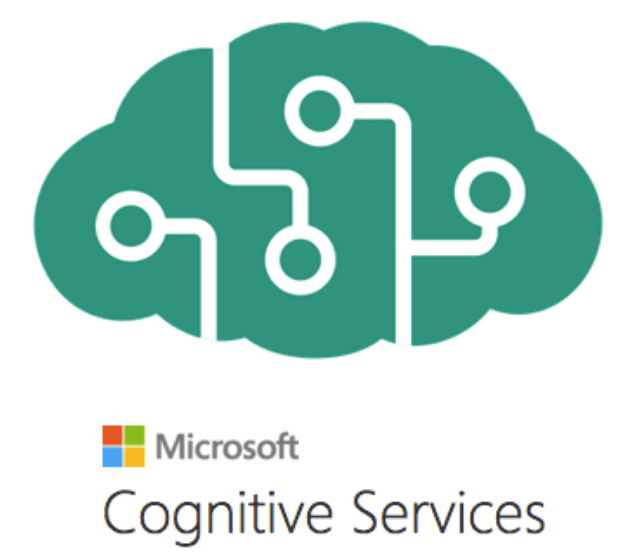
\includegraphics[scale=0.1,clip=true]{azure}
  \caption{Logo de Azure Cognitive Services}
  \label{fig:azure}
\end{figure}

La API del Translator Text de los Servicios Cognitivos de Microsoft proporciona las herramientas para lograr esto.

Para realizar la detección y traducción de idiomas, necesitamos utilizar la API del Translator Text. La API del Translator Text puede realizar la detección automática de idiomas, la traducción, la transliteración y las búsquedas de diccionarios bilingües. Admite más de 60 idiomas y Microsoft continúa agregando más \cite{chatbot4}.

Al escribir un chatbot que podría usarse en cualquier parte del mundo, las funciones le brindarán a su aplicación el soporte que necesita para comunicarse con cualquier usuario en su idioma nativo.
